% Options for packages loaded elsewhere
\PassOptionsToPackage{unicode}{hyperref}
\PassOptionsToPackage{hyphens}{url}
%
\documentclass[
  a4paper,
]{scrbook}

\usepackage{amsmath,amssymb}
\usepackage{lmodern}
\usepackage{iftex}
\ifPDFTeX
  \usepackage[T1]{fontenc}
  \usepackage[utf8]{inputenc}
  \usepackage{textcomp} % provide euro and other symbols
\else % if luatex or xetex
  \usepackage{unicode-math}
  \defaultfontfeatures{Scale=MatchLowercase}
  \defaultfontfeatures[\rmfamily]{Ligatures=TeX,Scale=1}
  \setmainfont[]{Latin Modern Roman}
  \setsansfont[]{Latin Modern Roman}
\fi
% Use upquote if available, for straight quotes in verbatim environments
\IfFileExists{upquote.sty}{\usepackage{upquote}}{}
\IfFileExists{microtype.sty}{% use microtype if available
  \usepackage[]{microtype}
  \UseMicrotypeSet[protrusion]{basicmath} % disable protrusion for tt fonts
}{}
\makeatletter
\@ifundefined{KOMAClassName}{% if non-KOMA class
  \IfFileExists{parskip.sty}{%
    \usepackage{parskip}
  }{% else
    \setlength{\parindent}{0pt}
    \setlength{\parskip}{6pt plus 2pt minus 1pt}}
}{% if KOMA class
  \KOMAoptions{parskip=half}}
\makeatother
\usepackage{xcolor}
\setlength{\emergencystretch}{3em} % prevent overfull lines
\setcounter{secnumdepth}{5}
% Make \paragraph and \subparagraph free-standing
\ifx\paragraph\undefined\else
  \let\oldparagraph\paragraph
  \renewcommand{\paragraph}[1]{\oldparagraph{#1}\mbox{}}
\fi
\ifx\subparagraph\undefined\else
  \let\oldsubparagraph\subparagraph
  \renewcommand{\subparagraph}[1]{\oldsubparagraph{#1}\mbox{}}
\fi


\providecommand{\tightlist}{%
  \setlength{\itemsep}{0pt}\setlength{\parskip}{0pt}}\usepackage{longtable,booktabs,array}
\usepackage{calc} % for calculating minipage widths
% Correct order of tables after \paragraph or \subparagraph
\usepackage{etoolbox}
\makeatletter
\patchcmd\longtable{\par}{\if@noskipsec\mbox{}\fi\par}{}{}
\makeatother
% Allow footnotes in longtable head/foot
\IfFileExists{footnotehyper.sty}{\usepackage{footnotehyper}}{\usepackage{footnote}}
\makesavenoteenv{longtable}
\usepackage{graphicx}
\makeatletter
\def\maxwidth{\ifdim\Gin@nat@width>\linewidth\linewidth\else\Gin@nat@width\fi}
\def\maxheight{\ifdim\Gin@nat@height>\textheight\textheight\else\Gin@nat@height\fi}
\makeatother
% Scale images if necessary, so that they will not overflow the page
% margins by default, and it is still possible to overwrite the defaults
% using explicit options in \includegraphics[width, height, ...]{}
\setkeys{Gin}{width=\maxwidth,height=\maxheight,keepaspectratio}
% Set default figure placement to htbp
\makeatletter
\def\fps@figure{htbp}
\makeatother

\usepackage{booktabs}
\usepackage{longtable}
\usepackage{array}
\usepackage{multirow}
\usepackage{wrapfig}
\usepackage{float}
\usepackage{colortbl}
\usepackage{pdflscape}
\usepackage{tabu}
\usepackage{threeparttable}
\usepackage{threeparttablex}
\usepackage[normalem]{ulem}
\usepackage{makecell}
\usepackage{xcolor}
\usepackage{titling}
\setlength{\droptitle}{-2cm}
\preauthor{
  \begin{center}
  \Large
  \vspace{10mm}
  by

  \vspace{20mm}
}
\postauthor{
  \end{center}
  \vfill
}

\predate{
  \begin{center}
  A thesis 
  submitted in fulfilment of the \\
  requirements of the degree of \\
  Doctor of Philosophy in Physics\\               % Degree
  School of Physical and Chemical Sciences\\          % Department
  Te Herenga Waka - Victoria University of Wellington\\                       % University 
  \vspace{5mm}
}
\postdate{
  \\
  
\includegraphics[width=3in,height=1.5in]{figures/VUW-logo.png}\\
  \end{center}
  }
\makeatletter
\makeatother
\makeatletter
\@ifpackageloaded{bookmark}{}{\usepackage{bookmark}}
\makeatother
\makeatletter
\@ifpackageloaded{caption}{}{\usepackage{caption}}
\AtBeginDocument{%
\ifdefined\contentsname
  \renewcommand*\contentsname{Table of contents}
\else
  \newcommand\contentsname{Table of contents}
\fi
\ifdefined\listfigurename
  \renewcommand*\listfigurename{List of Figures}
\else
  \newcommand\listfigurename{List of Figures}
\fi
\ifdefined\listtablename
  \renewcommand*\listtablename{List of Tables}
\else
  \newcommand\listtablename{List of Tables}
\fi
\ifdefined\figurename
  \renewcommand*\figurename{Figure}
\else
  \newcommand\figurename{Figure}
\fi
\ifdefined\tablename
  \renewcommand*\tablename{Table}
\else
  \newcommand\tablename{Table}
\fi
}
\@ifpackageloaded{float}{}{\usepackage{float}}
\floatstyle{ruled}
\@ifundefined{c@chapter}{\newfloat{codelisting}{h}{lop}}{\newfloat{codelisting}{h}{lop}[chapter]}
\floatname{codelisting}{Listing}
\newcommand*\listoflistings{\listof{codelisting}{List of Listings}}
\makeatother
\makeatletter
\@ifpackageloaded{caption}{}{\usepackage{caption}}
\@ifpackageloaded{subcaption}{}{\usepackage{subcaption}}
\makeatother
\makeatletter
\@ifpackageloaded{tcolorbox}{}{\usepackage[many]{tcolorbox}}
\makeatother
\makeatletter
\@ifundefined{shadecolor}{\definecolor{shadecolor}{rgb}{.97, .97, .97}}
\makeatother
\makeatletter
\makeatother
\ifLuaTeX
  \usepackage{selnolig}  % disable illegal ligatures
\fi
\usepackage[citestyle = ieee,urldate = iso8601]{biblatex}
\addbibresource{references.bib}
\IfFileExists{bookmark.sty}{\usepackage{bookmark}}{\usepackage{hyperref}}
\IfFileExists{xurl.sty}{\usepackage{xurl}}{} % add URL line breaks if available
\urlstyle{same} % disable monospaced font for URLs
\hypersetup{
  pdftitle={Volatile Organic Compound Detection Using Insect Odorant-Receptor Functionalised Field-Effect Transistors},
  pdfauthor={Eddyn Oswald Perkins Treacher},
  hidelinks,
  pdfcreator={LaTeX via pandoc}}

\title{Volatile Organic Compound Detection Using Insect Odorant-Receptor
Functionalised Field-Effect Transistors}
\author{Eddyn Oswald Perkins Treacher}
\date{Sep 2023}

\begin{document}
\frontmatter
\maketitle
\ifdefined\Shaded\renewenvironment{Shaded}{\begin{tcolorbox}[borderline west={3pt}{0pt}{shadecolor}, sharp corners, frame hidden, breakable, interior hidden, boxrule=0pt, enhanced]}{\end{tcolorbox}}\fi

\mainmatter
\bookmarksetup{startatroot}

\hypertarget{acknowledgements}{%
\chapter*{Acknowledgements}\label{acknowledgements}}
\addcontentsline{toc}{chapter}{Acknowledgements}

\markboth{Acknowledgements}{Acknowledgements}

\begin{verbatim}
69450
\end{verbatim}

Rifat, Alex - vapour sensor Erica Cassie - FET sensing setup Rob Keyzers
and Jennie Ramirez-Garcia - NMR spectra Patricia Hunt - Computational
chemistry

\bookmarksetup{startatroot}

\hypertarget{characteristics-of-pristine-carbon-nanotube-graphene-field-effect-transistors}{%
\chapter{Characteristics of Pristine Carbon Nanotube \& Graphene Field
Effect
Transistors}\label{characteristics-of-pristine-carbon-nanotube-graphene-field-effect-transistors}}

\begin{verbatim}
103704
\end{verbatim}

\hypertarget{carbon-nanotube-network-morphology}{%
\section{Carbon Nanotube Network
Morphology}\label{carbon-nanotube-network-morphology}}

Figure~\ref{fig-afm-morphology} shows a side-by-side comparison of the
surface morphology of carbon nanotube films fabricated using the methods
described in \textbf{?@sec-dep-carbon-nanotubes}. These images were
collected using an atomic force microscope and processed in the manner
described in \textbf{?@sec-afm-characterisation}. They each show bundles
of carbon nanotubes with a range of diameters and lengths, with each
bundle containing one or multiple nanotubes. As discussed in previous
works using solvent-based deposition techniques for depositing carbon
nanotubes, multi-tube bundles form due to strong mutual attraction
between nanotubes
\autocite{Zheng2017,Thanihaichelvan2018,Thanihaichelvan2019,Nguyen2021}.
However, when surfactants are present, they adsorb onto the carbon
nanotubes and form a highly repulsive structure able to overcome the
strong attraction between nanotubes. This repulsion then keeps the
individual carbon nanotubes isolated
\autocite{Wenseleers2004,Shimizu2013}. The diameter range provided by
the supplier for the individual carbon nanotubes used is 1.2-1.7 nm,
while the length range is 0.3-5.0 \(\mu\)m (Nanointegris).

\begin{figure}

\begin{minipage}[t]{0.47\linewidth}

{\centering 

\raisebox{-\height}{

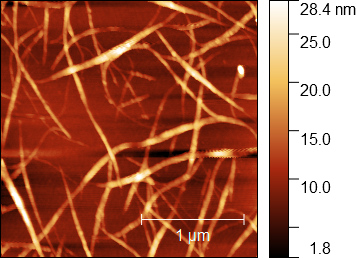
\includegraphics{./figures/ch5/Ned_NTQ24_20220125_00235.png}

}

}

\subcaption{\label{fig-bundled-network}Solvent-based deposition}
\end{minipage}%
%
\begin{minipage}[t]{0.05\linewidth}

{\centering 

~

}

\end{minipage}%
%
\begin{minipage}[t]{0.47\linewidth}

{\centering 

\raisebox{-\height}{

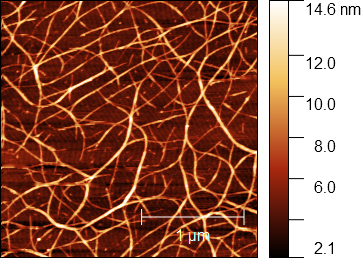
\includegraphics{./figures/ch5/Ned_NTQ8C7_w4_pristine_00084_20210428(2).png}

}

}

\subcaption{\label{fig-dropcast-network}Dropcast surfactant-based
deposition}
\end{minipage}%
\newline
\begin{minipage}[t]{0.26\linewidth}

{\centering 

~

}

\end{minipage}%
%
\begin{minipage}[t]{0.47\linewidth}

{\centering 

\raisebox{-\height}{

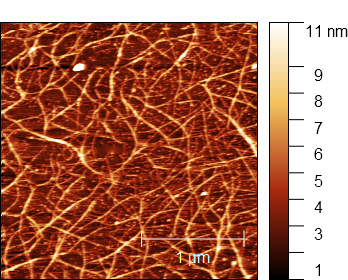
\includegraphics{./figures/ch5/Ned_NGQ14D2_W4_pristine_20220713_00567.png}

}

}

\subcaption{\label{fig-steaming-network}Steam-assisted dropcast
surfactant-based deposition}
\end{minipage}%
%
\begin{minipage}[t]{0.26\linewidth}

{\centering 

~

}

\end{minipage}%

\caption{\label{fig-afm-morphology}2.5 \(\mu\)m x 2.5 \(\mu\)m atomic
force microscope images of carbon nanotube films deposited using various
methods. NOTE NEED TO ADD EXAMPLES OF SURFACTANT BASED DEPOSITION
POST-ANNEALLING!!!}

\end{figure}

The distribution of the deposited carbon nanotubes was modelled to
quantatively understand the effect of the various methods used on the
resulting network morphology. The diameter range of deposited
single-walled carbon nanotubes can be modelled via a normal or Gaussian
distribution \autocite{Thanihaichelvan2018,Liu2013,Vobornik2023}.
However, when we extract and bin the height profiles from the 2.5
\(\mu\)m x 2.5 \(\mu\)m AFM images in Figure~\ref{fig-afm-morphology},
the histograms do not follow a normal distribution. The AFM histogram
shape results from the SiO\(_2\) substrate and carbon nanotubes both
exhibiting a degree of surface roughness, which is partially due to the
presence of atmospheric contaminants. In the case of the
surfactant-deposited networks, residual surfactant may also contribute
to surface roughness \autocite{Vobornik2023}.

It has been demonstrated that the surface roughness of a bare SiO\(_2\)
substrate can also be modelled with a normal distribution. This normal
distribution has a spread of approximately \pm1 nm about the mean, which
can be set as the reference or zero point for other height measurements
\autocite{Velicky2015}. As both the carbon nanotube and silicon dioxide
background heights can each be modelled using a normal distribution, we
therefore assume that a linear combination of normal distributions can
be used to model the AFM histograms in Figure~\ref{fig-afm-morphology}.

\begin{figure}

\begin{minipage}[t]{0.47\linewidth}

{\centering 

\raisebox{-\height}{

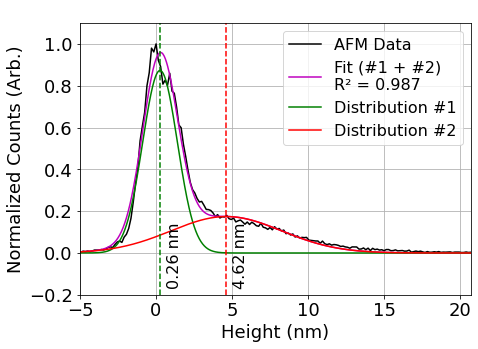
\includegraphics{./figures/ch5/Ned_NTQ24_20220125_00235_histogram.png}

}

}

\subcaption{\label{fig-bundled-network-histogram}Solvent based
deposition}
\end{minipage}%
%
\begin{minipage}[t]{0.05\linewidth}

{\centering 

~

}

\end{minipage}%
%
\begin{minipage}[t]{0.47\linewidth}

{\centering 

\raisebox{-\height}{

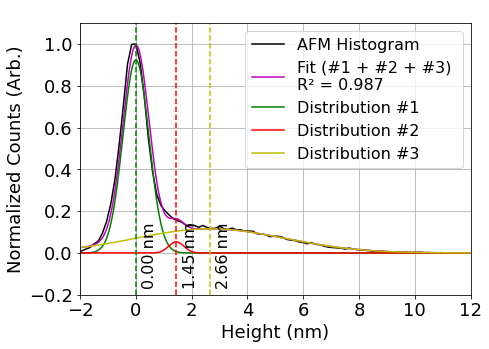
\includegraphics{./figures/ch5/Ned_NTQ8C7_w4_pristine_00084_20210428(2)_histogram.png}

}

}

\subcaption{\label{fig-dropcast-network-histogram}Dropcast
surfactant-based deposition}
\end{minipage}%
\newline
\begin{minipage}[t]{0.26\linewidth}

{\centering 

~

}

\end{minipage}%
%
\begin{minipage}[t]{0.47\linewidth}

{\centering 

\raisebox{-\height}{

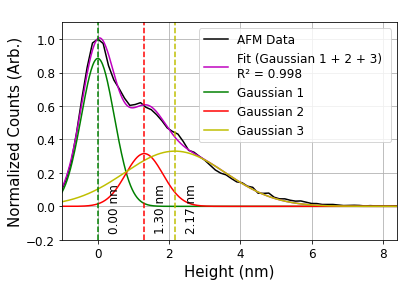
\includegraphics{./figures/ch5/Ned_NGQ14D2_W4_pristine_20220713_00567_histogram.png}

}

}

\subcaption{\label{fig-steaming-network-histogram}Steam-assisted
dropcast surfactant-based deposition}
\end{minipage}%
%
\begin{minipage}[t]{0.26\linewidth}

{\centering 

~

}

\end{minipage}%

\caption{\label{fig-afm-histograms}Surface profile histograms extracted
from the 2.5 \(\mu\)m x 2.5 \(\mu\)m atomic force microscope images seen
in Figure~\ref{fig-afm-morphology}, each fitted with a linear
combination of normal distributions. The component normal distributions
corresponding to each linear combination are also shown.}

\end{figure}

By using the analysis discussed in Section~\ref{sec-histogram-analysis},
we find that a linear combination of normal distribution fits to all
histograms corresponding to the AFM images in
Figure~\ref{fig-afm-morphology} with an R-squared value of at least
0.987. The first or left-most distribution for all three figures in
Figure~\ref{fig-afm-histograms} corresponds to the SiO\(_2\) substrate
roughness, centered at \(\sim\) 0 nm and with a standard deviation of
0.4-1.2 nm. For the carbon nanotube film deposited with solvent, the
second distribution then corresponds to bundles of carbon nanotubes. If
we model bundles as cylinders, and we assume the component nanotubes
follow 2D packing and are of equal diameter, we can give an estimate the
mean bundle size in terms of number of nanotubes \emph{n}
\autocite{Graham1998,Thanihaichelvan2018,Specht2023}.

\hypertarget{tbl-circle-packing}{}
\begin{longtable}[]{@{}
  >{\raggedright\arraybackslash}p{(\columnwidth - 16\tabcolsep) * \real{0.1053}}
  >{\raggedright\arraybackslash}p{(\columnwidth - 16\tabcolsep) * \real{0.1228}}
  >{\raggedright\arraybackslash}p{(\columnwidth - 16\tabcolsep) * \real{0.0965}}
  >{\raggedright\arraybackslash}p{(\columnwidth - 16\tabcolsep) * \real{0.0965}}
  >{\raggedright\arraybackslash}p{(\columnwidth - 16\tabcolsep) * \real{0.1228}}
  >{\raggedright\arraybackslash}p{(\columnwidth - 16\tabcolsep) * \real{0.1228}}
  >{\raggedright\arraybackslash}p{(\columnwidth - 16\tabcolsep) * \real{0.1228}}
  >{\raggedright\arraybackslash}p{(\columnwidth - 16\tabcolsep) * \real{0.1228}}
  >{\raggedright\arraybackslash}p{(\columnwidth - 16\tabcolsep) * \real{0.0877}}@{}}
\caption{\label{tbl-circle-packing}The first eight optimised ratios of
2D packed circle diameter to encompassing circle diameter, given to 3
s.f. (encompassing circle diameter = \(d\), number of packed circles =
\(n\), approximate packed circle diameter = \(d_n\)).\\
}\tabularnewline
\toprule()
\endhead
\(n\) & \text{2} & \text{3} & \text{4} & \text{5} & \text{6} & \text{7}
& \text{8} & \text{9} \\
\(d\)/\(d_n\) & \text{2.00} & 2.15 & 2.41 & \text{2.70} & \text{3.00} &
\text{3.00} & \text{3.30} & 3.61 \\
\bottomrule()
\end{longtable}

Table~\ref{tbl-circle-packing} shows the relationship between the
diameter of a bundle and the constituent diameters of up to nine 2D
packed carbon nanotubes within that bundle. The second distribution in
Figure~\ref{fig-bundled-network-histogram} indicates the mean diameter
of carbon nanotube bundles is 4.62 nm. Assuming an average carbon
nanotube diameter of 1.45 nm, we find a \(d\)/\(d_n\) packing ratio of
3.19, indicating an average bundle composition of \(\sim\) 7 nanotubes
in Figure~\ref{fig-bundled-network-histogram}.

For the carbon nanotube networks deposited using surfactant in
Figure~\ref{fig-afm-histograms}, we notice that there are two
non-SiO\(_2\) distributions present. The mean of the second
distribution, the left-most non-SiO\(_2\) distribution, falls below the
average height for a single carbon nanotube. This attribute indicates
that the distribution either represents broken pieces of individual
carbon nanotubes, residual surfactant or other atmospheric contamination
resistant to acetone and isopropanol rinsing. This contamination
distribution is significantly larger for the carbon nanotube devices
which used steam in the deposition process. The presence of this
contamination histogram distribution was consistently found for all
sampled surfactant-deposited film AFM data, while not present for any of
the sampled solvent-deposited films.

From Figure~\ref{fig-steaming-network}, we also see that steam deposited
devices have sparsely distributed \(\sim\) 10 nm high features visible
on their surface which are not present for the other films. These
observations may be evidence of trapped water microdroplets on the
surface from the steam, or could be from the steam causing surfactant to
form persistent features on the surface. The size of this central peak
may be useful for determining the extent of contamination in a carbon
nanotube film, discussed further in \textbf{?@sec-contamination}. Such
contamination may or may not have implications for biosensing
suitability, but surfactant contamination could certainly have negative
effects on biological elements sensitive to surfactant.

\hypertarget{tbl-histogram-parameters}{}
\begin{table}
\caption{\label{tbl-histogram-parameters}The mean of histogram distributions across three different samples for
carbon nanotube films deposited using various methods, along with the
mean sample coverage with bundles and mean proportion of multitubed
bundles present. The mean of the carbon nanotube bundle distribution is
shown with an estimate of the number of nanotubes that could pack into
the mean bundle size via 2D packing. }\tabularnewline

\centering
\begin{tabular}{>{\raggedright\arraybackslash}p{2cm}ccccc}
\toprule
\multicolumn{1}{c}{\textbf{ }} & \multicolumn{3}{c}{\textbf{Distribution Mean (nm)}} & \multicolumn{2}{c}{\textbf{Bundle Attributes}} \\
\cmidrule(l{3pt}r{3pt}){2-4} \cmidrule(l{3pt}r{3pt}){5-6}
 & Silicon & Contaminant & Bundles (tubes) & \% multi-tube & \% coverage\\
\midrule
Solvent deposited & 0.1 ± 2.3 & — & 6.2 ± 3.7 (13) & 78 ± 16 & 35 ± 21\\
 &  &  &  &  \vphantom{1} & \\
Surfactant deposited & 0.0 ± 0.4 & 1.0 ± 0.4 & 2.0 ± 1.8 (1) & 27 ± 25 & 31 ± 9\\
 &  &  &  &  & \\
Surfactant deposited with steam & 0.0 ± 0.5 & 1.3 ± 0.6 & 2.0 ± 1.2 (1) & 17 ± 17 & 50 ± 11\\
\bottomrule
\end{tabular}
\end{table}

The distribution means corresponding to each type of deposition method,
averaged across histogram fits from three 2.5 \(\mu\)m x 2.5 \(\mu\)m
atomic force microscope images, are given in
Table~\ref{tbl-histogram-parameters}. The carbon nanotube bundle mean is
given alongside the number of carbon nanotubes corresponding to the mean
height according to 2D packing as given in
Table~\ref{tbl-circle-packing} and Thanihaichelvan \emph{et al.}
\autocite{Thanihaichelvan2018}.

It is noticeable that the location of silicon and contamination
distribution means are highly consistent between films. Also notable is
a the large decrease in bundle size when surfactant is used in the
deposition process. There is also a large standard deviation in mean
bundle size seen for solvent deposited devices, corresponding to a wide
range of bundle sizes present on the atomic force microscope images of
the solvent-deposited films.

It is also important to consider that for all figures in
Figure~\ref{fig-afm-morphology}, larger height measurements in the
carbon nanotube distribution include surface contamination on the carbon
nanotubes as well as bundle-bundle junctions. The distribution may also
encompass broken nanotube pieces and some silicon oxide surface
contamination at the low end of the range. When considering the
proportion of single-tube bundles relative to multi-tube bundles, we
exclude heights from the carbon nanotube normal distribution below 1.2
nm, the minimum height of the supplied carbon nanotubes. We also exclude
heights above double the distribution mean, to ignore bundle-bundle
junctions and surface contamination.

We then compare the proportion of the curve below and above 2.9 nm, the
minimum multi-tube bundle size for 1.45 nm diameter nanotubes. By doing
so, we get a rough estimate of the proportion of single- to multi-tube
bundles present on the surface. We can also compare the total area of
the carbon nanotube distribution to the area of the other distributions
to get an estimate of the surface coverage by bundles. These values,
averaged across the histogram fits from three 2.5 \(\mu\)m x 2.5
\(\mu\)m atomic force microscope images, are given in
Table~\ref{tbl-histogram-parameters}. It should also be noted that
nanotubes undergo some compression from the AFM tip, so these values are
possibly underestimates. However, the mean values for
surfactant-deposited films are in line with those previously found for
IsoNanotubes-S deposited on silicon oxide using alternative analysis
methods \autocite{Vobornik2023}.

In Figure~\ref{fig-afm-morphology} and
Table~\ref{tbl-histogram-parameters}, we see that carbon nanotubes
deposited in a surfactant dispersion form bundles which are
significantly less wide than the bundles in the film deposited using
solvent. However, we also see that despite the presence of surfactant,
not all surfactant-dispersed carbon nanotubes are deposited
individually. Bundling may occur during the process of deposition onto
the substrate, which could disrupt the repulsive forces from the
surfactant coating and allow attractive forces to temporarily dominate.
The

It is possible that the bundling of surfactant-dispersed carbon
nanotubes occurs due to the coffee-ring effect
\autocite{Deegan1997,VanGaalen2021}. The coffee-ring effect refers to a
build-up of dispersed solid forming around the edges of a dispersion
evaporating on a surface. This process occurs due to the dispersion
edges being fixed by surface forces, leading to capillary flow outwards
to replace liquid evaporating at the edges, bringing solid material
along with it. The presence of vapour is known to disrupt this effect
\autocite{Bishop2020}. Table~\ref{tbl-histogram-parameters} demonstrates
that on average, the presence of steam reduces the number of nanotube
bundles present and increases surface coverage, supporting the above
hypothesis.

\hypertarget{sec-dummy-sensing}{%
\section{Salt Concentration Sensing with Phosphate Buffered
Saline}\label{sec-dummy-sensing}}

-nLOF2020 resist being used leads to devices with less drift!!

\appendix
\addcontentsline{toc}{part}{Appendices}

\hypertarget{sec-photolithography}{%
\chapter{Photolithography}\label{sec-photolithography}}

\begin{figure}

{\centering 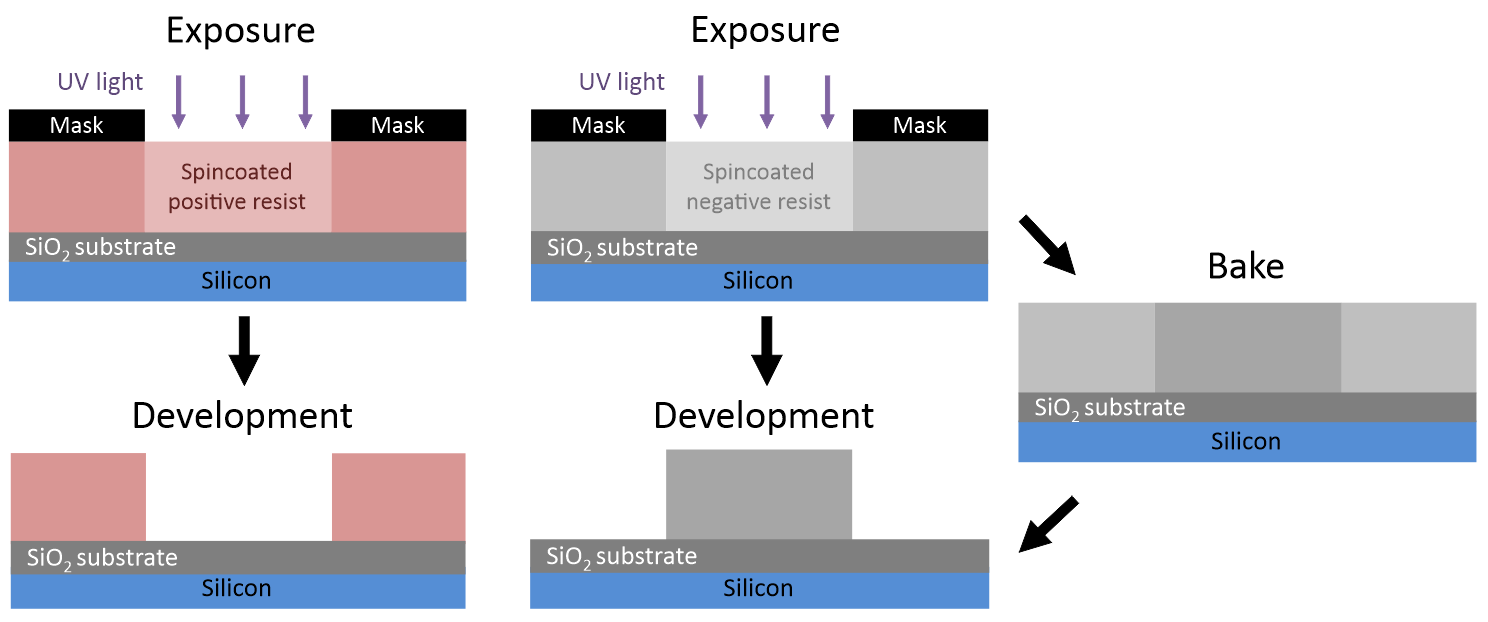
\includegraphics{./figures/app1/positive-negative-photolithography.png}

}

\caption{\label{fig-photolithography-types}A side-view comparison of
generic photolithography processes for positive and negative resists in
the ideal case. Photolithography with a positive resist requires a
single softbake step before exposure, while for negative resists a
second baking step is required after exposure (Thicknesses shown not to
scale).}

\end{figure}

This section details some of the standard photolithography procedures
used in the device fabrication processes detailed in
\textbf{?@sec-fabrication}. Photoresists, also referred to here as
``resists'', are UV light-sensitive polymeric resins used for
photolithography. Both positive and negative photoresists were used in
various fabrication processes. Positive resists are made soluble in
alkalines by UV light exposure, meaning exposed areas are removed in the
development process. Conversely, negative resists are cross-linked by
exposure and a post-exposure bake step. The unexposed areas of the
negative resist are then removed in the development process
\autocite{Microchemicals}. Figure~\ref{fig-photolithography-types} gives
a visual representation of these differences.

\begin{figure}

\begin{minipage}[t]{0.47\linewidth}

{\centering 

\raisebox{-\height}{

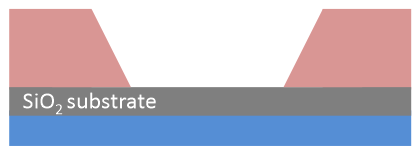
\includegraphics{./figures/app1/overcut-profile.png}

}

}

\subcaption{\label{fig-overcut-profile}Overcut profile of a positive
resist}
\end{minipage}%
%
\begin{minipage}[t]{0.05\linewidth}

{\centering 

~

}

\end{minipage}%
%
\begin{minipage}[t]{0.47\linewidth}

{\centering 

\raisebox{-\height}{

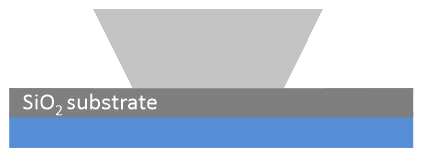
\includegraphics{./figures/app1/undercut-profile.png}

}

}

\subcaption{\label{fig-undercut-profile}Undercut profile of a negative
resist}
\end{minipage}%

\caption{\label{fig-photolithography-profiles}Two different resist
profiles seen for different types of photoresist. Each profile has had
the central region of the substrate exposed to UV light prior to
development. The undercut profile is ideal for thin-film metal
deposition and subsequent patterned removal, known as ``lift-off''.}

\end{figure}

The specific photoresist selected for photolithography depends on the
specific use case. The types used in this thesis are positive and
negative AZ\(^\circledR\) photoresists (AZ\(^\circledR\) 1518,
Microchemicals GmbH; AZ\(^\circledR\) nLOF 2020, Microchemicals GmbH)
and SU-8 (SU8-2150, Kayaku Advanced Materials, formerly Microchem). The
AZ\(^\circledR\) resists used here have a minimum film thickness of
\(1.5\textrm{ } \mu \textrm{m}\) \autocite{Microchemicals}, while the
SU8-2150 has a minimum film thickness of
\(0.5\textrm{ } \mu \textrm{m}\) \autocite{Kayaku}. Positive resists
which have not been thermally crosslinked will soften at higher
temperatures (\(\gtrsim 100^\circ\)C for AZ\(^\circledR\) 1518), leading
to a rounded profile. This is not the case for negative resists, which
are more thermally stable \autocite{Microchemicals}. Each resist
therefore has a different cross-section profile, as shown in
Figure~\ref{fig-photolithography-profiles}.

If metal deposition is performed on a positive resist, some metal can
collect on the outwardly-sloped sidewalls of the resist (see
Figure~\ref{fig-photolithography-profiles}) which forms significant
spikes on the edges of the deposited metal upon lift-off. On the other
hand, metal cannot collect on top of the inwardly-sloped negative
profile sidewalls, which avoids the formation of large edge spikes.
Therefore, the negative resist profile is more suited to metal or metal
oxide deposition and lift-off processes, though the process is more
sensitive to human error due to requiring more processing steps than
positive resist \autocite{Microchemicals}. Finally, when it is suitably
processed SU-8 is considered to be more stable and biocompatible than
other photoresists \autocite{Albarghouthi2022}. It is especially
biocompatible when chemically modified via processes such as isopropanol
sonication and O\(_2\) plasma treatment \autocite{Chen2021}.

All photolithographic exposure was performed using a Karl Suss MJB3
Contact Aligner with a USHIO super-high pressure 350 W mercury lamp
(USH-350DS, Japan). When performing photolithography, the intensity
reading from the aligner was 20.8 - 24.2 mW/cm\(^2\) (Note however that
an external photometer reading at 400 nm found an intensity output of
17.2 mW/cm\(^2\) when the aligner read 21.0 mW/cm\(^2\)).

In general, photolithography procedures should be performed under yellow
lighting, as light wavelengths from 320-450 nm can promote reactions in
the photoresist used. Aging of photoresist over time can also
significantly affect the photolithography process, and therefore all
processes should be re-optimised regularly over time to give the desired
result \autocite{Microchemicals}. The range in processing times for some
steps of the processes used here are largely due to the effects of aging
on the photoresist.

The step-by-step processes for each resist are detailed in the
subsequent sections.

\hypertarget{azcircledr-1518-photoresist}{%
\section{\texorpdfstring{AZ\(^\circledR\) 1518
photoresist}{AZ\^{}\textbackslash circledR 1518 photoresist}}\label{azcircledr-1518-photoresist}}

\begin{enumerate}
\def\labelenumi{\arabic{enumi}.}
\item
  Spincoat at a final speed of 4000 rotations per minute (rpm) for 1
  minute, with an initial acceleration of 500 rpm/s (notes: clean the
  substrate with acetone, isopropanol (IPA) and nitrogen before
  spincoating; use only the minimum amount of photoresist required to
  fully cover the wafer surface; avoid any gaps or bubbles in the
  photoresist).
\item
  Softbake 2-4 minutes at \(95^\circ\)C on the hotplate (2 min for
  individual devices, 4 min for a quarter wafer)
\item
  Mask expose for 10-12 s (note: clean mask with acetone/IPA and N\(_2\)
  dry before use)
\item
  Develop with 3 parts AZ\(^\circledR\) 326 (2.38 \% TMAH metal-ion free
  developer, Microchemicals GmbH) in 1 part deionised (DI) water for
  30-45 s (note: rinse for 10-15 s in one development solution, then
  perform the rest of the development in clean developer for a cleaner
  profile; lightly agitate the solution throughout the development
  process)
\item
  Rinse device for 30 s in DI water to remove excess developer, then dry
  under nitrogen
\end{enumerate}

\hypertarget{azcircledr-nlof-2020-photoresist}{%
\section{\texorpdfstring{AZ\(^\circledR\) nLOF 2020
photoresist}{AZ\^{}\textbackslash circledR nLOF 2020 photoresist}}\label{azcircledr-nlof-2020-photoresist}}

\begin{enumerate}
\def\labelenumi{\arabic{enumi}.}
\item
  Spincoat at final speed of 3000 rotations per minute (rpm) for 1
  minute, with an initial acceleration of 500 rpm/s (notes: clean the
  substrate with acetone, isopropanol (IPA) and nitrogen before
  spincoating; avoid any gaps or bubbles in the photoresist)
\item
  Softbake for precisely 60 s at \(110^\circ\)C on the hotplate
\item
  Mask expose for 2.7-3 s (note: clean mask with acetone/IPA and N\(_2\)
  dry before use)
\item
  Post-exposure bake for precisely 60 s at \(110^\circ\)C on the
  hotplate to cross-link exposed resist
\item
  Develop with 3 parts AZ\(^\circledR\) 326 in 1 part DI water for 60-70
  s (note: rinse for 30 s in one development solution, then perform the
  rest of the development in clean developer for a cleaner profile;
  lightly agitate the solution throughout the development process)
\item
  Rinse device for 30 s in DI water to remove excess developer, then dry
  under nitrogen
\end{enumerate}

\hypertarget{su8-2150-photoresist}{%
\section{SU8-2150 photoresist}\label{su8-2150-photoresist}}

\begin{enumerate}
\def\labelenumi{\arabic{enumi}.}
\item
  SU-8 was diluted in cyclopentanone until viscosity was low enough to
  spincoat on substrate and then sonicated at \(50^\circ\)C for 3-4
  hours (Note: The dilution ratio used was \textasciitilde1 part SU-8 to
  5 parts cyclopentanone. However, the age of the SU-8 may mean that
  significant evaporation had occurred prior to use, and the amount of
  SU-8 actually present is underrepresented by this ratio)
\item
  Spincoat first with a final speed of 500 rpm (acceleration 500 rpm/s)
  for 10 seconds, followed by spincoating at 4000 rpm (acceleration 7500
  rpm/s) for 40 s.
\item
  Softbake for 10 minutes at \(95^\circ\)C on the hotplate
\item
  Mask expose for 6-8 s (note: clean mask with acetone/IPA and N\(_2\)
  dry before use)
\item
  Post-exposure bake for 10 minutes at \(95^\circ\)C on the hotplate to
  cross-link exposed resist
\item
  Develop with SU-8 developer (Kayaku Advanced Materials, formerly
  Microchem) for 10-15 s, then clean in IPA for 30 s, repeat this step
  once then dry under nitrogen (note: lightly agitate the solution
  throughout the development process)
\end{enumerate}

\hypertarget{sec-python}{%
\chapter{Python Code for Data Analysis}\label{sec-python}}

\hypertarget{code-repository}{%
\section{Code Repository}\label{code-repository}}

The code used for general analysis of field-effect transistor devices in
this thesis was written with Python 3.8.8. Contributors to the code used
include Erica Cassie, Erica Happe, Marissa Dierkes and Leo Browning. The
code is located on GitHub and the research group OneDrive, and is
available on request.

\hypertarget{sec-histogram-analysis}{%
\section{Atomic Force Microscope Histogram
Analysis}\label{sec-histogram-analysis}}

The purpose of this code is to return morphology statistics such as
height distribution and carbon nanotube coverage/density from atomic
force microscope (AFM) images of carbon nanotube networks. The code uses
the SciPy optimize package to fit two or three normal distributions to
.xyz datasets from AFM images processed in Gwyddion (see
\textbf{?@sec-afm-characterisation}). The number of normal distributions
was chosen based on which gave a better quality fit to the .xyz data. It
was originally designed by Erica Happe in Matlab, and adapted by Marissa
Dierkes and myself for use in Python.

The .xyz data is initially sorted into bins with 0.15 nm size. The bin
with the maximum number of counts is set at 0 nm, as this peak
represents the mean of the surface roughness of the bare silicon. The
fitting parameters \(m_1\), \(s_1\), \(k_1\), \(m_2\), \(s_2\), \(k_2\)
(as well as \(m_3\), \(s_3\), \(k_3\) for three normal distributions)
are used in the objective function Equation~\ref{eq-lin-combo-gaussian}
when optimising.

\begin{equation}\protect\hypertarget{eq-lin-combo-gaussian}{}{
f(x) = k_1\exp{\Bigg(-\frac{{(x-m_1)}^{2}}{{2s_1}^{2}}\Bigg)} + k_2\exp{\Bigg(-\frac{{(x-m_2)}^{2}}{{2s_2}^{2}}\Bigg)} + ...
}\label{eq-lin-combo-gaussian}\end{equation}

These fitting parameters represent the mean (m), standard deviation (s)
and amplitude (k) of each normal distribution. We can find the initial
guess for these fitting parameters by using the histogram data to
roughly approximate these values. \(k_1\) is taken as the maximum
y-value of the data being fitted, \(m_1\) is set to zero and \(s_1\) is
taken as one-third of the difference between \(m_1\) and the x-value of
the first datapoint where the y-value is greater than 1\% of \(k_1\). We
find the Gaussian given by these values, and subtract it from the
existing dataset. We then take \(k_2\) to be the maximum y-value of this
modified dataset, and \(m_1\) to be the x-value of the maximum y-value.
\(s_2\) is taken as the difference between \(m_1\) and the x-value of
the first datapoint where the y-value is greater than 60\% of \(k_2\).
This process is repeated to find \(k_3\) and \(m_3\), and \(s_3\) is
one-third of the difference between \(m_3\) and the x-value of the
\emph{last} datapoint where the y-value is greater than 1\% of \(k_3\).
In this iterative manner, we find a reasonably good initial guess for
our fit.

Using the objective function with these fitting parameters in the
scipy.optimize.curve\_fit module, we receive optimised fitting
parameters which gave an R-squared value of 0.96 or greater. By
calculating the area under each of the normal distributions found from
the fit, we can find the proportion of the surface covered by carbon
nanotube bundles. The code also allows for discretely binning continuous
data from fitted normal distributions and examining the proportion of
counts above or below a particular height.

\hypertarget{vapour-delivery-system}{%
\chapter{Vapour Delivery System}\label{vapour-delivery-system}}

\hypertarget{technical-notes}{%
\section{Technical Notes}\label{technical-notes}}

Two LabView Virtual Instruments (VIs) were adapted from pre-existing VIs
for operating the mass flow controllers and monitoring vapour flow into
the device chamber, as well as monitoring temperature and humidity in
the vapour delivery system's manifold. These VIs were named ``\,'' A
third VI was developed in parallel which combined the first two Virtual
Instruments, alongside allowing the sequence of values to control the
mass flow controllers.

From Honours report: ``\,``\,'' Figure 12 gives the right side of the
front panel of the LabView VI sample with vapour.VI, which letsus preset
an autonomously-performed vapour sensing sequence. Each row in each
array module corresponds to a differennest step in this sequence. The
`howManySteps' module lets us set how many of these steps are performed.
The `Durations Array' module determines the length of time in seconds
each step is performed over. The `Carrier Flows Array' and `Dilution
Flows Array' modules let us set the carrier flow and dilution flow,
respectively, in standard cubic centimetres per minute (sccm) through
the gas rig at each step. The carrier flow pushes analyte vapour into
the vapour-sensing device chamber, while dilution flow is used to modify
the flow behaviour of the analyte vapour entering the chamber. The
vapour sensing sequence as depicted in Figure 12 was used for all vapour
sensing runs in this investigation. At the end of the sequence, the data
collected about the vapour sensing process was saved as an .lvm file.
``\,``\,''

\hypertarget{future-improvements}{%
\section{Future Improvements}\label{future-improvements}}


\backmatter
\printbibliography


\end{document}
